\section{Transfer learning}
%\cite{Taylor2009TransferSurvey}.
Transfer learning involves the use of experience gained when learning one or more tasks, to improve the performance on a different but related task. Each task is represented by a Markov Decision Process (MDP).\\  Here, we discuss a framework for transfer methods that can be used for reinforcement learning, closely following \cite{Taylor2009TransferSurvey}.\\

As already said, the transfer of knowledge always happens between one or more source tasks and a target task. First, an appropriate set of tasks must be selected. Afterwards, the transfer learning algorithm must learn how these source tasks are related to the target task. Then, the appropriate knowledge can be transferred.\\

\subsection{Transfer learning dimensions} % (fold)
\label{sub:transfer_learning_dimensions}
Transfer learning can differ in 5 major aspects. Here we will discuss each of them.\\

To be able to transfer knowledge, some assumptions must be made about differences between the source tasks and the target task. This can be for example in the underlying dynamics of the environment, which can make the task harder or easier to solve, or different sets of possible actions at certain states. These differences define between which type of source and target tasks knowledge can be transferred. The differences between the source task(s) and target task can also make the knowledge transfer easier or harder, requiring the appropriate guidance by a human or a method that can overcome these differences in case of a fully autonomous transfer learner.\\
Multi-task learning is a special kind of task learning where the problems for the source and target tasks are drawn from the same distribution instead of having arbitrary source and target tasks. More specifically, the transition function is drawn from a fixed distribution of functions. For the mountain car environment, this may mean for example that the motor of the car differs in power in different tasks.\\

As was stated, first the set of source tasks needs to be selected. Again, this can be done by a human in case of a human-guided scenario. However, the selection may also be done by the agent itself. For example, it can learn multiple source tasks and then use them all for transfer. Another possibility is to select the source tasks that are the most relevant and lead to highest performance for the target task. The agent may also just aim to avoid negative transfer, such that the specific selection of source tasks does not to worsen learning performance for the target task.
The agent could also modify the source task(s) such that the transferred knowledge is the most useful in the target task.\\

Instead of just knowing that tasks are related, many methods also need to know how tasks are related, using task mappings. This is necessary to make the knowledge gained on the source tasks useful for the target task. Tasks may differ in state and action variables and the in the semantic meaning of them. In the mountain car environment, one can have a task where the goal is on the opposite side. As such, taking the action \texttt{Left} has a different meaning for these tasks. Actions in the two tasks must be mapped such that their effects are similar.\\
Again, these mappings can be provided by a human or they can be learned by the agent. Note that these mappings may be partial and not every action in the source task is mapped to an action in the target task or vice-versa. For the state space, it is also possible to map the states themselves instead of the state variables.\\
In multi-task learning, states and variables are the same and have the same meaning. Because of this, no task mappings are necessary in multi-task learning.\\

Task learning methods can also differ in the type of knowledge that is transferred between source and target tasks. This knowledge can be for example an action-value function, transitions or policy gradient parameters. For tasks that are closely related, detailed knowledge may be useful. Otherwise, high-level information may result in a better learning performance. The type of knowledge that is transferred can also depend on the type of source and target tasks and on the task mappings.\\

Last, the task learning method may also restrict which reinforcement learning algorithms that can be used. It is possible for example that only a class of reinforcement learning algorithms or only one specific reinforcement learning algorithm can be used with the task learning method or that the algorithm is the same for both the source and target tasks. Ideally, the reinforcement learning algorithms can be chosen freely and may be selected based on the characteristics of the task at hand.\\
% subsection transfer_learning_dimensions (end)

\subsection{Metrics}
\label{sub:tl_metrics}
Several metrics exist to evaluate the learning performance and solution quality of transfer learning algorithms. Generally, one metric does not give a complete representation of the overall performance of the algorithm. Because of this, often multiple metrics are used.\\
Here we will list the most popular ones:
\begin{itemize}
    \item \textit{Jumpstart}: This is the initial improvement that the target task has over an algorithm that doesn't use knowledge transfer. However, no learning has occurred yet. Because of this, learning performance can't be measured. The metric also does not give an indication about the final performance, i.e. the performance after having learned.
    \item \textit{Asymptotic performance}: This is the opposite of \textit{jumpstart} performance and measures the performance improvement after having learned the target task. However, this is hard to measure because one has to know when the task learning algorithm converged. Furthermore, the task learning algorithm and the algorithm that doesn't use knowledge transfer may require a different training time in order to converge.
    \item \textit{Total reward}: This is the total reward that the algorithm has accumulated during learning, i.e. the area under the learning curve. In case of improvement, this area is bigger than when transfer learning isn't used. This can be achieved when the transfer learning algorithm has a higher learning rate. However, convergence is again an issue here. An algorithm that learns slower and thus takes more time to converge may accumulate a higher total reward than a faster algorithm, although the latter may even reach a higher performance. This metric is only useful for task that always have the same duration.
    \item \textit{Transfer ratio}: This is the ratio of the total reward improvement that the transfer learning algorithm has over the other algorithm. Because it uses the \textit{total reward} metric, it suffers from the same issues. Furthermore, it is also influenced by the reward structure. For example, an agent always receiving a reward of $+1$ at the end of the episode may result in a different ratio.
    \item \textit{Time to threshold}: This measures the time needed to reach a pre-defined performance. A transfer learning algorithm may need less time to reach this threshold. The threshold needs to be defined manually and depends on the task domain and learning method.
\end{itemize}
A graph with 3 of the 5 metrics is shown in Figure~\ref{fig:TLmetrics}.
\begin{figure}[htb]
    \centering
    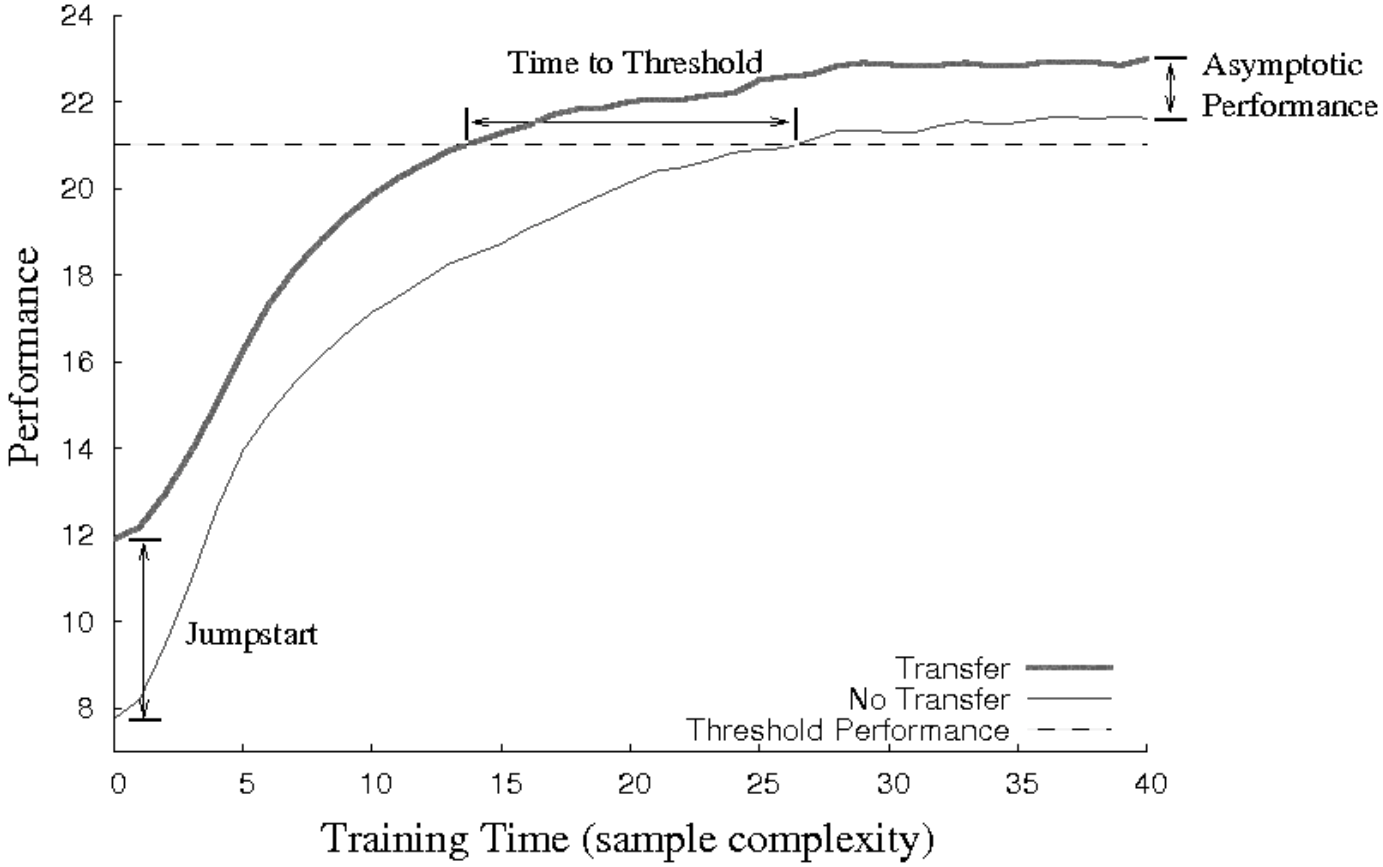
\includegraphics[width=\linewidth]{images/tlmetrics.png}
    \caption[Transfer learning metrics]{A graph comparing the \textit{jumpstart}, \textit{time to threshold} and \textit{asymptotic performance} metrics between the algorithm that uses knowledge transfer and the one that doesn't. Note that here the transfer learning algorithm performs better on all three metrics. It can also be seen that the total reward is higher. Source: \cite{Taylor2009TransferSurvey}.}
    \label{fig:TLmetrics}
\end{figure}
Instead of comparing the transfer learning algorithm with a algorithm that doesn't use knowledge transfer, it is also possible to compare the algorithm with the performance of humans (by averaging their performances). However, metrics must be chosen carefully such that they don't favor the algorithm or the human and they can be abused.

\subsection{Using Task Features for Zero-Shot Knowledge Transfer in Lifelong Learning}
An extra problem is to learn multiple variations of environment instead of just one. This means that for each of these tasks the transition function is slightly different, while keeping the same action space and state space.
In \cite{Isele2016UsingLearning}, a method is presented that learns these task simultaneously by using a predefined description for each task.
When a new task arrives along with its features, obtained from its task descriptor, a policy can be generated that immediately results in a good performance, even though the algorithm was not applied on that task before and the task descriptor, task order and task distribution was not known on beforehand. This way, knowledge transfer can take place without the need of training data to identify relationships across tasks. For each subsequent task, the policy and feature vector are iteratively improved.\\
%factorization: ontbinding in factoren: bijv. 15=3*5
First, it is assumed that the policy parameters for every task $t$ can be factorized using a shared knowledge base $L \in \mathbb{R}^{d \times k}$: $\theta^{(t)} = Ls^{(t)}$. $s^{(t)} \in \mathbb{R}^{(k)}$ are the sparse coefficients over the basis, i.e. the latent representation of the policy's parameters for task $t$. $L$ is able to capture relationships among policies as this is used to compute every policy, whereas there is a sparse representation for computed for each task separately.\\
The features of the task are obtained by (possibly non-linear) feature extractors applied on the descriptor of the task: $\phi(m^{(t)}) \in \mathbb{R}^{d_m}$. These features can also be linearly factorized using another shared knowledge base $D \in \mathbb{R}^{d_m \times k}$: $\phi(m^{(t)}) = Ds^{(t)}$, where the same sparse representation is used as the one used to compute the policy. Both knowledge bases provide information about the task and because of this they share the same coefficient vectors $S$. We then used coupled dictionary optimization techniques from the sparse coding literature to optimize these dictionaries. They are updated iteratively based on trajectories samples from the current task.\\
When a new task arrives, with its task descriptor, we search for the coefficients $s^{(t_{new})}$ that minimize the difference between the extracted features and the reconstruction of it using the shared knowledge base $D$. Using these coefficients, we can compute the policy parameters using $\theta = Ls^{(t_{new})}$. Afterwards, we can iterate again to improve the sparse representation $s$ and the knowledge bases.
